\documentclass{sig-alternate-br}

\bibliographystyle{plain}

\usepackage{placeins}
%\floatbarrier
\usepackage{caption}
\captionsetup{labelfont=bf,font=bf}
\usepackage{subcaption}

\usepackage{listings}
\lstset{	numbers=left,
		escapechar=$,
		breaklines=true,
		numbersep=3pt}


\newtheorem{definition}{Definition}
\newtheorem{lemma}{Lemma}

\title{Proving correctness of Lace using interactive theorem prover tools}
\author{
	\alignauthor
	Thijs van Ede\\
	\affaddr{University of Twente}\\
	\affaddr{P.O. Box 217, 7500AE Enschede}\\
	\affaddr{The Netherlands}\\
	\affaddr{t.s.vanede@student.utwente.nl}\\
}
\date{\today}

\begin{document}
\maketitle

\section{UPDATE}
This week I started writing the introduction, which still needs a part on the background information. Perhaps, some explanation that is now at the Method section will be moved to the background information section. I wrote a new part on the method information about the order of linearisation points, and made some flow diagrams to illustrate this. The theorems to be proven are specified as invariants. Furthermore, I began documenting some proofs for Lace, which I will continue doing over the next week. When I've finished the documentation of the proof of Lace, I will start writing the conclusion and make some final additions to the paper. That is what I am planning to do this week. Furthermore, I made an appointment with my supervisor to show my progress and ask some questions.

\begin{abstract}
Interactive theorem prover tools 
\end{abstract}

\section{Introduction}
Modern day processors' multi-core architecture has increased demand for concurrent programming to fully utilise the processing power.
These concurrent programs need to be proven correct to ensure the desired execution.
Several methods for proving programs correct exist such as separation logic\cite{reynolds2002} and first-order logic\cite{smullyan1995}.

Interactive theorem prover tools such as Isabelle\cite{paulson1994isabelle}, Coq\cite{coq2015}, and PVS\cite{owre1992pvs} use various methods of logical based proving check models.
These tools are helpful in proving properties of both sequential\cite{badban2005verification} and concurrent\cite{colvin2006formal} \cite{shankar1993verification} algorithms.
The theorem prover tool PVS uses several decision procedures and a symbolic model checker, in combination with a random tester to help generating formal proofs.

This paper tries to proof several properties of the Lace algorithm\cite{vanDijk2014206} to illustrate the method of proving concurrent programs.
Lace is a concurrent algorithm for thread scheduling among processors.
Its use of a memory fence, compare-and-swap system call and both concurrent and sequential components make it an ideal algorithm to proof correct.

In this paper, we will prove the Lace algorithm correct using the interactive theorem prover tool PVS.
The algorithm is modeled by constructing linearisation points where the state of the system changes, and using them to generate a flow diagram of the program.
Subsequently, PVS assists in proving the required invariants using this model in combination with several assumptions about the system.
With the invariants a comprehensive proof of the Lace algorithm is constructed.

\subsection{Background information}

\section{Preliminaries}
\subsection{System}
This paper assumes the algorithm runs on a shared memory system with the x86 memory model.
This memory model allows the reordering of loads before stores, that is, write operations are buffered before they are stored in memory.
Thus threads might read old values, even though they have been written by other threads.
These writes may not have become globally visible yet, because they are still buffered.
Memory fences are used to flush these write buffers and make changes globally visible.
Memory stores are immediately visible to threads that wrote them, hence they do not require memory fences.

\subsection{Compare-and-swap}
A compare-and-swap (\texttt{cas}) ensures thread safety by simulating an atomic memory operation.
The \texttt{cas} operation takes three parameters as input, namely a \texttt{variable}, an \texttt{expected value}, and a \texttt{replacement value}.
The \texttt{cas} operation compares the value of \texttt{variable} to the \texttt{expected value}. When those values are equal, the \texttt{replacement value} replaces the current value of \texttt{variable} and \texttt{cas} returns \texttt{true}.
If they are not equal, \texttt{variable} retains its current value and \texttt{cas} returns \texttt{false}.
Because of its atomicity, \texttt{cas} ensures only one thread executes successfully when multiple threads invoke \texttt{cas} with the same valid parameters.
\texttt{cas} is used for concurrent programming as it ensures thread safety and provides feedback to executing threads on whether their operation succeeded or not.

\subsection{Linearisation points}
\label{sec:lin}
An important aspect of proving concurrent algorithms is defining linearisation points\cite{herlihy1990}.
These linearisation points are the points in time the state of the system changes.
When reasoning about concurrent programs, information about the state of the system is needed to predict its expected behaviour.
By defining linearisation points, the order in which they occur can be varied and thereby all possible states can be derived.
That is, by varying the order of linearisation points, all possible equivalent sequential programs can be derived, which in turn can be reasoned about.

\subsection{Assumed properties}
First of all, we have four ways of classifying a task.
\begin{definition}A task x exists $\iff$ x < \texttt{head}\end{definition}
\begin{definition}A task x is stolen $\iff$ x < \texttt{tail}\end{definition}
\begin{definition}A task x is shared $\iff$ x < \texttt{split}\end{definition}
\begin{definition}A task x is private $\iff$ x $\geq$ \texttt{split}\end{definition}
In proving Lace correct, this paper assumes there is only one owner thread per deque and a possibly infinite number of thieving threads.
In practice there are more than one owner threads since there are multiple deques, however, the proof of correctness for one deque is equivalent to all other deques.
I.e. we assume that owner threads are not influenced by each other, only by thieving threads.

The second assumption is that thieving threads only call \texttt{steal} and the owner threads only calls \texttt{push}  and \texttt{pop}.
This implies that the owner thread is also the only thread that has access to \texttt{grow\_shared}  and \texttt{shrink\_shared}, since they are only called in \texttt{push} and \texttt{pop}.

In addition, this paper assumes the number of calls to \texttt{pop} is equal to the number of calls to \texttt{push} when the algorithm finished executing. I.e. the deque is empty when the program finished.

Finally, all deque values - i.e. tail, split, head, and the entries within the deque - are all set to zero when the deque is initialised.
\begin{figure}[h]
	\begin{enumerate}
		\setlength{\itemsep}{-3pt}
		\item One owner thread per deque.
		\item Possibly infinite number of thieving threads per deque.
	
		\item \texttt{steal} is only called by thieving threads.
		\item \texttt{push} and \texttt{pop} are only called by owner thread.
		\item Owner thread only calls \texttt{grow\_shared} and \texttt{shrink\_shared}.
	
		\item Number of \texttt{pop} calls $\leq$ number of \texttt{push} calls.
		\item When finished, number of \texttt{pop} calls = number of \texttt{push} calls.
	
		\item On initialisation all deque variables are set to zero.
	\end{enumerate}
	\caption{Assumed properties of Lace}
\end{figure}

\subsection{Required properties}
Lace requires some properties to work correctly.
First of all, the variables \texttt{head}, \texttt{split}, and \texttt{tail} should stay within bounds.
Figure \ref{inv:bounds} expresses this requirement as invariants. 
\begin{figure}[h]
	\texttt{0 $\leq$ head $\leq$ size}\\
	\texttt{0 $\leq$ split $\leq$ head}\\
	\texttt{0 $\leq$ tail $\leq$ head}
	\caption{Invariants: variables stay within bounds.}
	\label{inv:bounds}
\end{figure}
Furthermore, a task must be stolen only once, and executed exactly once.
To prove these properties, they are written as invariants.
When every task is stolen only once, it means thieving threads can only steal tasks $\geq$ \texttt{tail} and that when tail reduces, a task cannot be stolen again. The former part of the property is trivial, if tail increases it steals an unstolen task which is consistent with the requirement. The latter part is less trivial, if tail reduces, a stolen task cannot be executed again, therefore the stolen tasks need to be removed before tail is reduced. This is written as an invariant in Figure \ref{inv:stolen}.
\begin{figure}[h]
	\texttt{tail.new > tail.old || (tail.new $\leq$ tail.old \&\& tail.old == head \&\& pop() == STOLEN, head)}
	\caption{Invariant: every task is stolen only once.}
	\label{inv:stolen}
\end{figure}
To elaborate on this invariant: either \texttt{tail} increases when a new task is stolen, or \texttt{tail} decreases but the task has to be removed from the deque so that it cannot be stolen again.
When a task is executed once, this implies it is only stolen once and not executed by the owner thread, or it is executed by the owner thread and never stolen. This can be written as the invariant in Figure \ref{inv:exec}.
\begin{figure}[h]
	\texttt{(pop() == STOLEN \&\& head.new < head.old) || (pop() == WORK \&\& head.new < head.old)}
	\caption{Invariant: every task is executed only once.}
	\label{inv:exec}
\end{figure}

\section{Method}
In proving a concurrent program such as Lace correct, the linearisation points of the algorithm must be appointed.
For each of these linearisation points, the preconditions can be defined, keeping in mind the variables that can change because of concurrency.
By altering the order in which the linearisation points occur, each possible state of the system can be derived.
From here conclusions can be drawn about the desired behaviour of the system and its possible behaviour.

The first step of appointing linearisation points is trivial and could be done automatically.
However, because the algorithm is relatively simple and to illustrate how these points can be identified it is done manually.
First all global variables of the algorithm are identified, then each point in the algorithm where a variable is changed is appointed as a linearisation point.

The second step of defining the preconditions of each linearisation point is less trivial and for illustrative purposes they are also deduced manually.
In this case, the preconditions consist of the state of the system before the linearisation point.
This can be derived by the variables that are adjusted before the linearisation can occur and that cannot change due to other linearisation points.
Either because other linearisation points do not modify the variable or because the linearisation points that do modify it do not occur.

After the preconditions are established, the linearisation point will alter the state of the system, from this it is possible to calculate the postconditions.
However, due to concurrency, linearisation points can occur in different possible sequences, which will result in different outcomes for the state of the system.
Conclusions are drawn from these states, which will result in the invariants that are necessary to prove the system works correctly.
That is if it is possible to find invariants that state \texttt{tail.old $\leq$ tail.new || (tail.old == head \&\& pop() \&\& tail.new $\leq$ head)} and \texttt{(tail.old $\leq$ tail.new \&\& pop() == STOLEN) || pop() == WORK \&\& tail < head}.

To find out how threads and their manipulation of deque variables influence the distribution of work in the deque, the Lace algorithm has to be studied carefully.
This part will mainly be a literature research, the Lace algorithm is described in detail in \cite{vanDijk2014206}.
When the algorithm is modeled in PVS, an even more clear view ill become apparent on the influence of variables on the deque.

In proving Lace correct, we propose to model the Lace algorithm in the interactive theorem prover tool PVS\cite{owre1992pvs}. 
Here, the algorithm must be mapped to a series of mathematical lemma's, theorems, and functions.
Furthermore, the desired outcome must be expressed in set of theorems.
In the case of Lace, these theorems include a task being executed once, and the task always giving the same result, independent of the process that executes it.
After the algorithm has been modeled, PVS assists in generating a proof for the desired outcome.
This is done by applying formal logic to the given formulas.
Interactive theorem prover tools indicate whether the given model is enough to prove the algorithm correct.
If not, it provides missing theorems that needs to be proven by the user to prove the entire algorithm correct.

Various interactive theorem prover tools may be used for proving this algorithm correct.
However, this paper suggests to use the PVS 6.0 Allegro Lisp Binary for a Linux Intell 64-bit machine.
The model of the algorithm is constructed from its description in the paper \cite{vanDijk2014206}.

A proof constructed with an interactive theorem prover such as PVS holds in all cases and could also be constructed without using PVS.
The tool only helps to construct the proof and formalise the method of proving algorithms correct.
PVS will therefore speed up the process of constructing a proof and increase confidence in the proof.
It also increases the transferability of this research since the tool constructs equal proofs in an identical way.

\section{Modeling Lace}
A model for the Lace algorithm is constructed from its specifications as described in \cite{vanDijk2014206} and displayed in Figure \ref{fig:Lace}.
Note the that Figure \ref{fig:Lace} projects a slightly different form of the algorithm.
However, this alternate form is used to construct a model for Lace.
First of all, a model is created from the algorithm without the \texttt{allstolen} flag.

\subsection{Linearisation Points}
In Lace, the state of the system is dependent on the variables head, split, and tail.
The linearisation points are defined on these variables and can be found in Table \ref{tab:head}, \ref{tab:split}, and \ref{tab:tail} respectively.
Note that the variables used at linearisation points to change the state of the system are read at a point before they are used.
Thus the value might have changed when the program reaches the linearisation point, in which case it still uses the old value.

In addition to these three main variables, the algorithm also uses a \texttt{movesplit} and \texttt{allstolen} variable.
These variables influence the behaviour of the system by indicating whether the split point must be moved or all public tasks are stolen respectively.
Therefore, these variables are also included in the linearisation points, which can be found in Table \ref{tab:move}, \ref{tab:allst}, and \ref{tab:oallst}.

\subsubsection{Head}
\label{sec:head}
The head variable is modified in both the push and the pop methods.
Table \ref{tab:head} shows an overview of the linearisation points and the places where the variables used in the linearisation points are initialised.
The first linearisation point is at line 13 of Lace as shown in Figure \ref{fig:Lace}, where head is incremented by 1.
In this case the variable head is read in the same line of code but does not occur simultaneously with the write operation.
The second and third linearisation points are at line 45 and 47 of Lace as shown in Figure \ref{fig:Lace} respectively.
In both cases, head is decreased by 1 and the variable is read in the same line of code as it is written.
As with the first point, the read and write operation do not occur simultaneously.

\subsubsection{Split}
In Lace, the variable split has two instances, namely split and o\_split.
The latter instance of split is private, and thus visible to the owner thread but not to thieving threads.
To avoid confusion, split and o\_split are displayed in Table \ref{tab:split} and Table \ref{tab:osplit} respectively.
Just as explained in section \ref{sec:head} these tables indicate the methods, linearisation points, operations, initialisation points, and variables for the variable scrutinised, in this case the split and o\_split variables.
As opposed to the linearisation points of the variable head, split has linearisation points in which variables are used that are read in a different line of the algorithm.
This might indicate a greater chance of the variables being altered before they are used.

\subsubsection{Tail}
The final variable of the deque that is important to include in the model is tail, its linearisation points can be found in Table \ref{tab:tail}.
This variable is modified in the steal and push functions at lines 5 and 15 respectively.
In steal, tail is read at line 3 whilst incremented at line 5.
Because of this gap tail can be modified in the meantime by other threads.
The same goes for the modification of tail in the push method, since read and write do not occur simultaneously.

\subsubsection{Movesplit}
Movesplit is not part of the deque, but it indicates whether the owner thread should grow the shared part of the deque.
This boolean variable is set to true at line 8 of the algorithm and is set to false at lines 16 and 25.
These linearisation points can be found in Table \ref{tab:move}.

\subsubsection{Allstolen}
As with split, the variable \texttt{allstolen} has two instances, namely \texttt{allstolen} and \texttt{o\_allstolen}.
The global boolean variable \texttt{allstolen} is set to false at line 17 of the algorithm and to true at line 39.
The private \texttt{o\_allstolen} is set to false and true at lines 19 and 40 respectively.
The linearisation points can be found in Table \ref{tab:allst} and \ref{tab:oallst}.

\begin{table}[h]
	\begin{subtable}[h]{0.45\textwidth}
		\centering
		\begin{tabular}{|l|l|l|l|l|}
			\hline
			\textbf{method} & \textbf{lin pt} & \textbf{op} & \textbf{init pt} & \textbf{var} \\ \hline
			push            & 13                 & head+1      & 13                  & head               \\ \hline
			pop             & 45                 & head-1      & 45                  & head               \\ \hline
			pop             & 47                 & head-1      & 47                  & head               \\ \hline
		\end{tabular}
		\caption{Linearisation points of head variable.}
		\label{tab:head}
	\end{subtable}
	\hfill
	\begin{subtable}[h]{0.45\textwidth}
		\centering
		\begin{tabular}{|l|l|l|l|l|}
			\hline
			\textbf{method} & \textbf{lin pt} & \textbf{op} & \textbf{init pt} & \textbf{variables}  \\ \hline
			push            & 15                 & head        & 15                  & head                \\ \hline
			gr\_shared    & 23                 & (o+h+1)/2      & 22                  & o\_split,head \\ \hline
			shr\_shared  & 30                 & (t+s)/2      & 27                  & tail,split             \\ \hline
			shr\_shared  & 36                 & (t+s)/2      & t:32,s:27        & tail,split             \\ \hline
		\end{tabular}
		\caption{Linearisation points of split variable.}
		\label{tab:split}
	\end{subtable}
	\hfill
	\begin{subtable}[h]{0.45\textwidth}
		\centering
		\begin{tabular}{|l|l|l|l|l|}
			\hline
			\textbf{method} & \textbf{lin pt} & \textbf{op} & \textbf{init pt} & \textbf{variables}  \\ \hline
			push            & 18                 & head        & 18                  & head                \\ \hline
			gr\_shared    & 24                 & (o+h+1)/2      & 22                  & o\_split,head \\ \hline
			shr\_shared  & 37                 & (t+s)/2      & 27         & tail,split             \\ \hline
			shr\_shared  & 37                 & (t+s)/2      & t:32,s:27                  & tail,split             \\ \hline
		\end{tabular}
		\caption{Linearisation points of o\_split variable.}
		\label{tab:osplit}
	\end{subtable}
	\hfill
	\begin{subtable}[h]{0.45\textwidth}
		\centering
		\begin{tabular}{|l|l|l|l|l|}
			\hline
			\textbf{method} & \textbf{lin point} & \textbf{op} & \textbf{init point} & \textbf{variables} \\ \hline
			steal           & 5                  & t+1         & 3                   & tail           \\ \hline
			push            & 15                 & head-1      & 15                  & head               \\ \hline
		\end{tabular}
		\caption{Linearisation points of tail variable}
		\label{tab:tail}
	\end{subtable}
	\begin{subtable}[h]{0.45\textwidth}
		\centering
		\begin{tabular}{|l|l|l|l|l|}
			\hline
			\textbf{method} & \textbf{lin point} & \textbf{op} & \textbf{init point} & \textbf{variables} \\ \hline
			steal           & 8                  & true        & 8                   & movesplit          \\ \hline
			push            & 16                 & false       & 16                  & movesplit          \\ \hline
			grow\_shared    & 25                 & false       & 25                  & movesplit          \\ \hline
		\end{tabular}
		\caption{Linearisation points of movesplit variable}
		\label{tab:move}
	\end{subtable}
	\begin{subtable}[h]{0.45\textwidth}
		\centering
		\begin{tabular}{|l|l|l|l|l|}
			\hline
			\textbf{method} & \textbf{lin point} & \textbf{op} & \textbf{init point} & \textbf{variables} \\ \hline
			push            & 17                 & false       & 17                  & allstolen          \\ \hline
			shrink\_shared  & 39                 & true        & 39                  & allstolen          \\ \hline
		\end{tabular}
		\caption{Linearisation points of allstolen variable}
		\label{tab:allst}
	\end{subtable}
	\begin{subtable}[h]{0.45\textwidth}
		\centering
		\begin{tabular}{|l|l|l|l|l|}
			\hline
			\textbf{method} & \textbf{lin point} & \textbf{op} & \textbf{init point} & \textbf{variables} \\ \hline
			push            & 19                 & false       & 19                  & o\_allstolen       \\ \hline
			shrink\_shared  & 40                 & true        & 40                  & o\_allstolen       \\ \hline
		\end{tabular}
		\caption{Linearisation points of o\_allstolen variable}
		\label{tab:oallst}
	\end{subtable}
	\caption{ The method column indicates the method where the variable is modified. Lin pt column refers to the linearisation point in the Lace algorithm as shown in Figure \ref{fig:Lace}. The op column explains the executed operation. The init pt column refers to the point in the Lace algorithm where the variables are read. The final column var declares the variables that are used to modify variable. Note that in \ref{tab:split} and \ref{tab:osplit} o\_split and head are abbreviated to o, h respectively. Tail and split are abbreviated to t and s since these is a local variables as in the algorithm.}
\end{table}

\subsection{Preconditions}
For all initialisation points, some preconditions about the state of the system can be assumed.
In this section, the preconditions for each initialisation point as described in section \ref{sec:lin} are defined and substantiated.

\subsubsection{Head}
The first thing to note about \texttt{head} is that it is only modified from within the methods \texttt{push} and \texttt{pop}.
It is also assumed that these methods are only called from within the owner thread, implying there is no interference on that variable from other threads.
The first instance of \texttt{head} being modified is at line 13 of the algorithm in the method \texttt{push}.
Before the modification, line 11 checks whether \texttt{head == size}, if this is the case the method returns \texttt{FULL} and thus will not reach line 13.
Therefore, at the linearisation point of line 13 it is certain that \texttt{head} does not equal \texttt{size}.

At line 45 in the method \texttt{pop}, \texttt{head} is decremented.
At line 43 the method checks whether \texttt{head == 0}, if so the method returns.
In combination with the assumption that the number of pops never exceed the number of pushes, we derive that at this point, head must be larger than 0.
Because the if statement in line 44 must be true to reach line 45, \texttt{o\_allstolen} is true, or \texttt{o\_split == head} and \texttt{shrink\_shared()} returns true.
The method \texttt{shrink\_shared} only returns true after it set \texttt{allstolen} and \texttt{o\_allstolen}.
In combination with the assumption that both of these variables can only be adjusted by the owner thread, these will not change.
Therefore at the linearisation point of \texttt{head} at line 45, \texttt{o\_allstolen} is set.

At line 47 in \texttt{pop}, \texttt{head} is also decremented.
When this case appears, \texttt{o\_allstolen} is false and either \texttt{o\_split != head} or \texttt{shrink\_shared} returned false or both.
From this we conclude that \texttt{o\_allstolen} is not set.
//TODO check whether all variables needed are covered.

\subsubsection{split}
As with \texttt{head}, \texttt{split} and \texttt{o\_split} can also only be modified within the methods reachable by the owner, in this case \texttt{push}, \texttt{grow\_} \texttt{shared}, and \texttt{shrink\_shared}.
At the first linearisation point at line 15, \texttt{o\_allstolen} is set and \texttt{head} $\geq 1$.
The latter statement is true since the number of \texttt{pop} calls do not exceed the number of \texttt{push} calls, and \texttt{head} is incremented by 1 at line 13.

At the second linearisation point at line 23, \texttt{movesplit} is set.
Since \texttt{grow\_shared} is only called when movesplit is set and movesplit cannot be unset by any other thread than the owner, 

At the third linearisation point at line 30, \texttt{t} $\neq$ \texttt{s}, note that these are the local values initialised at line 27.
Thus \texttt{tail} and \texttt{split} can be altered.

The linearisation point at line 36 also implies \texttt{t} $\neq$ \texttt{s}, because of the if-statement at line 33.
The memory fence at line 31 secures the knowledge that \texttt{tail} is not modified until the memory fence is .

\subsubsection{tail}
\texttt{tail} is modified by both thieving threads and the owner thread.
Notably, the first linearisation point of \texttt{tail} is at line 5 of the algorithm, where tail is increased.
This modification uses the compare-and-swap method, which only executes if the given values are equal.
In this case the values \texttt{t} and \texttt{s} read at line 3 must be equal to the current values of \texttt{tail} and \texttt{split} respectively.
If this occurs, it can have two causes: neither values have changed, or the values have changed but are restored to their original state between line 3 and 5 of the algorithm.

At the second linearisation point at line 15, the flag \texttt{o\_allstolen} is set, since this is the only way to reach this part of the code and \texttt{o\_allstolen} is only modified by the owner thread itself.
Additionally, \texttt{head} is not equal to size, and incremented by 1 relative to line 13.

\begin{table}[h]
	\begin{subtable}[h]{0.45\textwidth}
		\centering
		\begin{tabular}{|l|l|l|}
			\hline
			\textbf{lin point} & \textbf{head}  & \textbf{allstolen} \\ \hline
			13                 & $\neq$ size       &                    \\ \hline
			45                 & \textgreater 0 & true               \\ \hline
			47                 & \textgreater 0 & true               \\ \hline
		\end{tabular}
		\caption{Preconditions head variable}
		\label{tab:init.head}
	\end{subtable}
	\hfill
	\begin{subtable}[h]{0.45\textwidth}
		\centering
		\begin{tabular}{|l|l|l|l|l|}
			\hline
			\textbf{lin point} & \textbf{head} & \textbf{tail}  & \textbf{split} & \textbf{allstolen} \\ \hline
			5                  &               & t=tail         & s=split        &                    \\ \hline
			15                 & $\neq$size    & \textgreater 0 & true           & true               \\ \hline
		\end{tabular}
		\caption{Preconditions points tail variable}
		\label{tab:init.tail}
	\end{subtable}
	\caption{Full caption}
\end{table}



\subsection{Order of linearisation points}
By assuming only one owner thread exclusively calls methods \texttt{push} and \texttt{pop}, all variables manipulated only at those methods will occur in order.
Subsequently, this is true for all methods \texttt{grow\_shared} and \texttt{shrink\_shared} which are invoked only through \texttt{push} and \texttt{pop}.
The natural order of linearisation points called by \texttt{push} and \texttt{pop} can be derived by creating a flow diagram.
In this section, the order of linearisation points for \texttt{push} and \texttt{pop} are derived respectively.

First of all, the method \texttt{push} has a flow diagram as depicted in Figure \ref{fig:push}.
Here the first linearisation point is at line 13, where head is increased.
If \texttt{o\_allstolen} is set, the program continues with linearisation point 15.
Then, if \texttt{movesplit} is true, it is set to false, otherwise it continues flowing through all linearisation points down to linearisation point 19 where \texttt{o\_allstolen} is set to false.
Alternatively, when \texttt{o\_allstolen} is false at line 14 and \texttt{movesplit} is true at line 20, it invokes the method \texttt{grow\_shared} which is depicted as the right part of the flow diagram.
\begin{figure}[h]
	\centering
	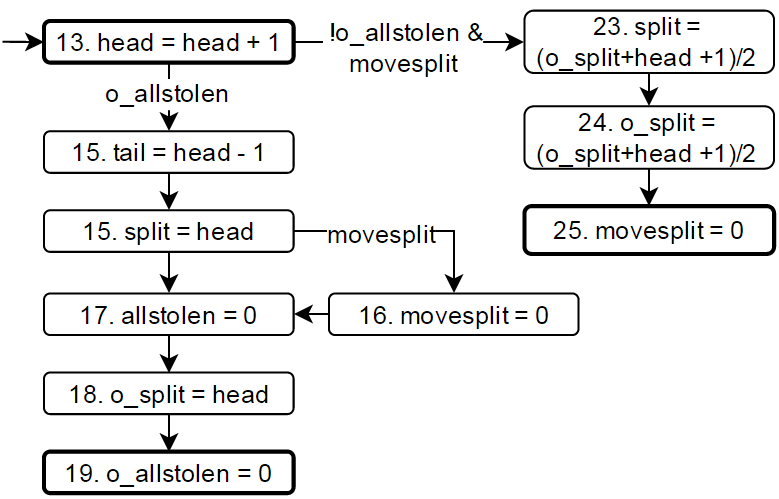
\includegraphics[scale=0.35]{Push_flow_diagram_2.png}
	\caption{Flow diagram of method push.}
	\label{fig:push}
\end{figure}

Second, the method \texttt{pop} has a flow diagram as depicted in Figure \ref{fig:pop}.
This diagram is less trivial than the \texttt{push} flow diagram.
Since the method \texttt{pop} first checks whether head equals 0 and returns when it does the linearisation points are not reached, thus the first condition of \texttt{head $\neq$ 0} is introduced.
After this, it checks whether \texttt{o\_allstolen} is set, if this is the case, it continues to decrease head and returns.
Alternatively, if \texttt{o\_allstolen} is false, it checks whether \texttt{o\_split == head}, if so, it calls the method \texttt{shrink\_shared} following the rhombus' upper arrow.
The method \texttt{shrink\_shared} first checks whether the variables \texttt{t} and \texttt{s} that it read from \texttt{tail} and \texttt{split} respectively are equal.
If this condition is true, it sets \texttt{allstolen} and \texttt{o\_allstolen} after which it returns true and continues at \texttt{pop}.
Subsequently, if the condition is false, it modifies \texttt{split} and sets a memory fence, depicted with the dashed lines.
After reading the \texttt{tail} variable into \texttt{t} again, the algorithm checks whether \texttt{t} equals \texttt{s}.
When they are equal, the method sets the \texttt{allstolen} variables, and returns true, after which it continues at \texttt{pop}.
However, when they are not equal, \texttt{t} and the temporary variable \texttt{new\_s} are compared.
If \texttt{t $>$ new\_s}, \texttt{split} is modified, otherwise only \texttt{o\_split} is set to \texttt{new\_s}.
Thereafter, the method returns false and continues at \texttt{pop}.
\begin{figure}[h]
	\centering
	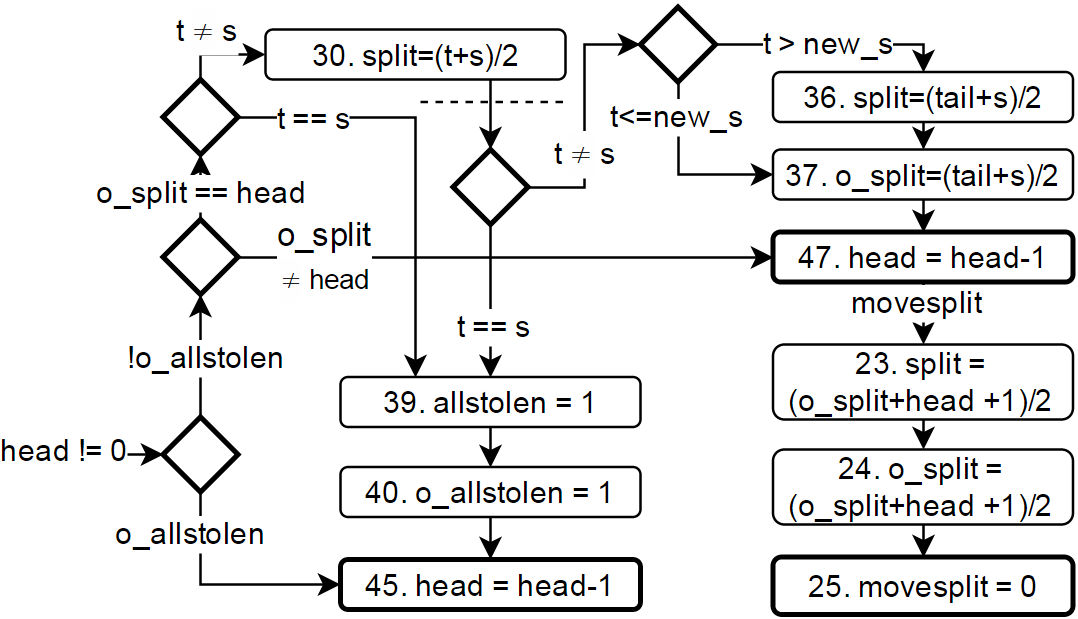
\includegraphics[scale=0.25]{Pop_flow_diagram_2.png}
	\caption{Flow diagram of method pop.}
	\label{fig:pop}
\end{figure}

From these flow diagrams, the possible sequences of linearisation points are clear.
Note that the linearisation points modified by thieving threads through the method \texttt{steal} are not included.
Since these occur at arbitrary points in the algorithm, it does not make sense to include them in a flow chart.

\section{Proving Lace}
\begin{lemma}
	\texttt{head $\leq$ size}.
	\label{lem:headsize}
\end{lemma}
\begin{proof}
	Table \ref{tab:head} indicates \texttt{head} is only increased at method \texttt{push}.
	Since it is assumed \texttt{head} = 0 at the start of the algorithm, i.e. \texttt{head} < \texttt{size}, it is left to prove the linearisation point cannot be reached if \texttt{head $\geq$ size}.
	In PVS we input the code as depicted in Figure \ref{pvs:head}.
	To proof lemma \texttt{lemma\_head}, we use axioms \texttt{head\_start}, stating \texttt{head} < \texttt{size} at the initialisation, and \texttt{head\_size} stating \texttt{head $\neq$ size}, i.e. line 11 of Lace.
	Then, we expand function \texttt{incr\_head(head)}, which increases \texttt{head} by 1, i.e. line 13 of Lace.
	Then using PVS' grind option, it concludes that indeed the lemma holds.
\end{proof}
\begin{figure}[h]
	\texttt{head\_start: AXIOM head < size}\\
	\texttt{head\_size: AXIOM NOT (head = size)}\\
	\texttt{incr\_head(head): posnat = head+1}\\
	\texttt{lemma\_head: LEMMA incr\_head(head) <= size}
	\caption{PVS proof of head $\leq$ size}
	\label{pvs:head}
\end{figure}

\begin{lemma}
	\texttt{head $\geq$ 0}
	\label{lem:headzero}
\end{lemma}
\begin{proof}
	Table \ref{tab:head} indicates \texttt{head} is only decreased at the method \texttt{pop}.
	From the flow diagram we find that to reach a linearisation point where \texttt{head} is decreased, \texttt{head $\neq$ 0}.
	In PVS we input the code as depicted in Figure \ref{pvs:headzero}.
	Here we use the axiom \texttt{head\_start} to denote that the starting position of \texttt{head} is 0, or in this case $\geq$ 0.
	The axiom \texttt{head\_zero} states, \texttt{head} $\neq$ 0, as line 43 of Lace indicates.
	To proof \texttt{lemma\_head}, we introduce both axioms and expand the method \texttt{decr\_head} after which we use PVS' grind option.
	This concludes that indeed the lemma holds.
\end{proof}
\begin{figure}[h]
	\texttt{head\_start: AXIOM head >= 0}\\
	\texttt{head\_zero: AXIOM NOT (head = 0)}\\
	\texttt{decr\_head(head): posnat = head-1}\\
	\texttt{lemma\_head: LEMMA func\_decr(head) >= 0}
	\caption{PVS proof of head $\geq$ 0}
	\label{pvs:headzero}
\end{figure}

\begin{lemma}
	\texttt{allstolen = o\_allstolen} at linearisation points of global variables from the owner thread.
\end{lemma}
\begin{proof}
	Table \ref{tab:allst} and \ref{tab:oallst} indicate that both \texttt{allstolen} variables only change through methods \texttt{push} and \texttt{shrink\_shared}. Figure \ref{fig:push} states that private variable \texttt{o\_split} is the only variable to change in between the modifications of the \texttt{allstolen} variables. Subsequently, Figure \ref{fig:pop} states there are no linearisation between the modifications at all.
\end{proof}

\begin{lemma}
	\texttt{shrink\_shared} returns \texttt{True} $\Rightarrow$ \texttt{allstolen} and \texttt{o\_allstolen}.
\end{lemma}
\begin{proof}
	Table \ref{tab:allst} and \ref{tab:oallst} indicate both \texttt{allstolen} variables can only be modified within the methods \texttt{push} and \texttt{shrink\_shared}. Since both can only be called by the owner thread, they cannot be run simultaneously.  Thus, only \texttt{shrink\_shared} needs to be inspected. The return \texttt{true} statement of \texttt{shrink\_shared} corresponds to linearisation point 40 in Figure \ref{fig:pop}, since no more linearisation points occur between that point and the return true statement. Therefore, the code depicted in Figure \ref{pvs:shrshared} is used to proof the \texttt{allstolen} variables are set when \texttt{shrink\_shared} returns true. By adding lemmas \texttt{allstolen\_set} and \texttt{o\_allstolen\_set} to the proof, and using PVS' \texttt{grind} option, the tool verifies both \texttt{allstolen} flags are set to true if \texttt{shrink\_shared} returns true.
\end{proof}
\begin{figure}
	\texttt{allstolen\_set: AXIOM allstolen}\\
	\texttt{o\_allstolen\_set: AXIOM o\_allstolen}\\
	\texttt{shr\_shared\_ret: LEMMA allstolen AND o\_allstolen}
	\caption{PVS proof of shrink\_shared $\Rightarrow$ allstolen \&\& o\_allstolen}
	\label{pvs:shrshared}
\end{figure}

\begin{lemma}
	\texttt{tail.new $\geq$ tail.old or\\(tail.new < tail.old} and \texttt{tail.old-tail.new $\leq$ \#pop())}
\end{lemma}
\begin{proof}
	The first part of the lemma states that \texttt{tail} should increase, this is true for all linearisation points except at line 15 of Lace, as described in Table \ref{tab:tail}.
	The second part states, that if \texttt{tail} is decreased, the method \texttt{pop} must have returned \texttt{STOLEN} and on modification, \texttt{tail.old} must have been equal to \texttt{head}.
	The only possibility for \texttt{tail} to decrease is at line 15 of Lace, where it is set to \texttt{head-1}, see Table \ref{tab:tail}.
	As Figure \ref{fig:push} shows the linearisation point of line 15 can only be reached if \texttt{o\_allstolen} is set.
	
\end{proof}

\begin{lemma}
	\texttt{pop()} $\iff$ \texttt{head.new = head.old - 1}
\end{lemma}
\begin{proof}
	Table \ref{tab:head} shows \texttt{head = head-1} can only be invoked from within the method \texttt{pop}, hence \texttt{head.new = head.old-1 $\Rightarrow$ pop()} holds.
	Figure \ref{fig:pop} shows it is impossible to go from linearisation point 45 to 47 or vise versa. Furthermore, the Figure shows both linearisation points are the first possible end states to reach. Therefore \texttt{pop() $\Rightarrow$ head.new = head.old -1} holds.
\end{proof}

\begin{figure}
\begin{lstlisting}
def steal():
  if allstolen: return NOWORK
  (t,s) = (tail,split) $\emph{\#t, s are local}$
  if t < s:
    if cas((tail,split), (t,s), (t+1,s)):
      return WORK(t)
    else: return NONE $\emph{\#busy}$
  elif not movesplit: movesplit = 1
  return NONE $\emph{\#no work}$
\end{lstlisting}
\begin{lstlisting}[firstnumber=10]
def push(data):
  if head == size: return FULL
  $\emph{\#write task data at deque head}$
  head = head + 1
  if o_allstolen:
    (tail,split) = (head-1,head)
    if movesplit: movesplit = 0
    allstolen = 0
    o_split = head
    o_allstolen = 0
  elif movesplit: grow_shared()
\end{lstlisting}
\begin{lstlisting}[firstnumber=21]
def grow_shared():
  new_s = (o_split+head+1)/2
  split = new_s
  o_split = new_s
  movesplit = 0
\end{lstlisting}
\begin{lstlisting}[firstnumber=26]
def shrink_shared():
  (t,s) = (tail,split)
  if t != s:
    new_s = (t+s)/2
    split = new_s
    MFENCE
    t = tail $\emph{\#read again}$
    if t != s:
      if t > new_s:
        new_s = (t+s)/2
        split = new_s
      o_split = new_s
      return FALSE
  allstolen = 1
  o_allstolen = 1
  return TRUE
\end{lstlisting}
\begin{lstlisting}[firstnumber=42]
def pop():
  if head == 0: return EMPTY, None
  if o_allstolen or (o_split == head and shrink_shared()):
    head = head-1
    return STOLEN, head
  head = head-1
  if movesplit: grow_shared()
  return WORK, head
\end{lstlisting}
\caption{Lace algorithm as described in "Lace: Non-blocking Split Deque for Work-Stealing"\cite{vanDijk2014206}}
\label{fig:Lace}
\end{figure}

\bibliography{Bibliography}

\end{document}